%%===========================================================%%
%%                                                           %%
%%                          EXPERIMENTAL SETUP                          %%
%%                                                           %%
%%===========================================================%%


\chapter{Experimental setup}\label{chap:experimentalsetup}
Measurement of diffractive events requires many subdetectors of the STAR experiment \cite{Ackermann:2002ad}, whose scheme is drawn in the Figure \ref{fig:starscheme}.
The main part of the~STAR detector is the TPC, the tracking detector, which provides information about momentum  and ionization energy loss $dE/dx$ of charged particles with $p_T \geq 100$~MeV/c in the full azimuthal coverage $\left(0\leq \phi \leq 2\pi\right)$ and a~pseudorapidity coverage of $-1.2 \lesssim \eta \lesssim 1.2$. The particle identification (PID) capability of the STAR experiment was improved by the Time-Of-Flight (TOF) system \cite{Llope:2009zz},  which measures TOF with resolution of about $100$~ps. 
\begin{figure}[hb]
	\centering
	
	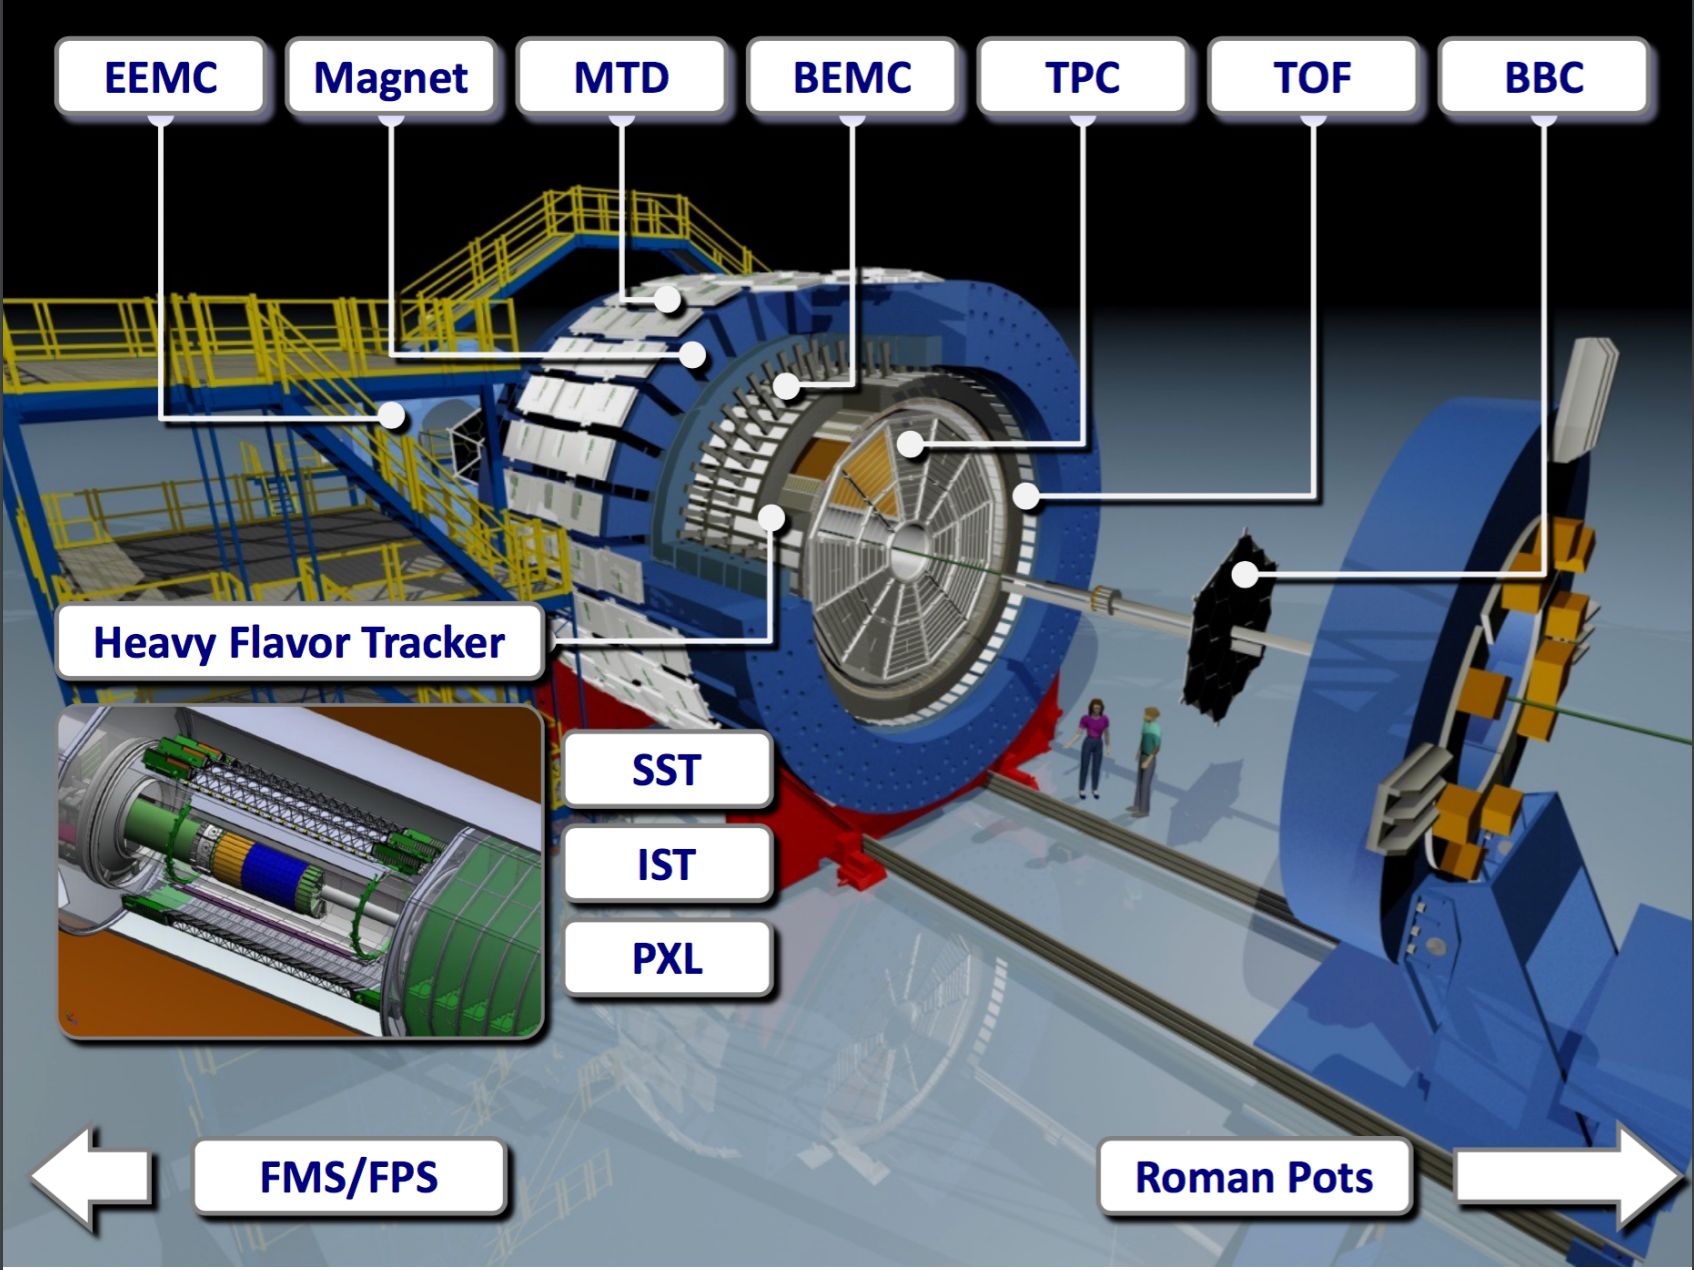
\includegraphics[width=0.9\linewidth]{graphics/experimentalSetup/star.png}
	
	\caption[Perspective view of the STAR detector, with a cutaway for viewing inner detector systems as configured in 2015.]{ Perspective view of the STAR detector, with a cutaway for viewing inner detector systems as configured in 2015.}
	\label{fig:starscheme}
\end{figure}

System of forward detectors in STAR \cite{A_N}, whose scheme is drawn in the Figure \ref{fig:rpscheme}, consists of  four stations of the Roman Pots (RP), two of each placed symmetrically with respect to the Interaction Point (IP), with two Silicon Strip Detector (SSD) packages in each station. The stations are located between RHIC DX and D0 dipole magnets at distances $15.8$ and $17.6$~m from  the IP. Each SSD package, housed inside the RP vessel, consists of four silicon planes and the~scintillator counters used for triggering. The acceptance of the RPs limits the kinematics of the protons to the~values of squared four-momentum transfer (Mandelstam $t$), $0.03\leq -t \leq 0.3$~GeV$^2/$c$^{2}$, and fractional momentum loss of the proton $\xi<0.6$.

\begin{figure}[hb]
	\centering
	
	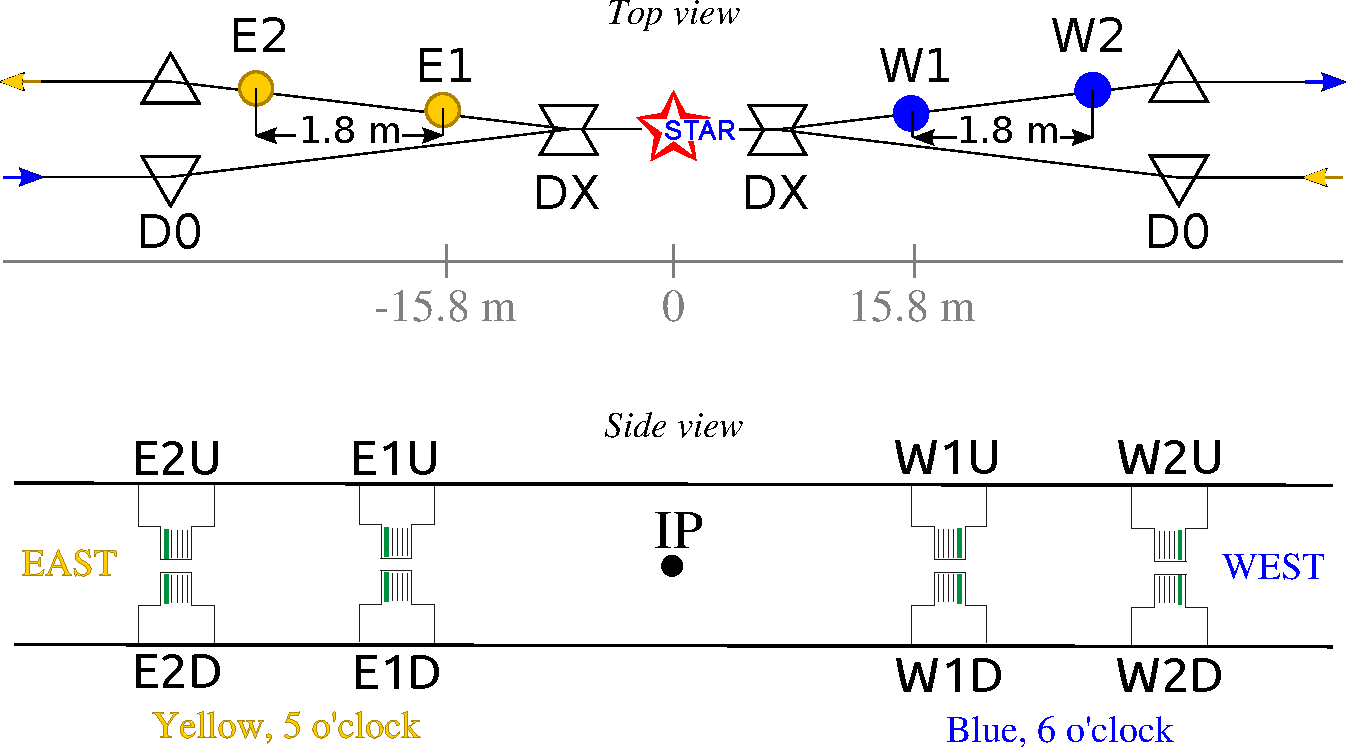
\includegraphics[width=\linewidth, page=1]{graphics/experimentalSetup/RP_phaseII_2.pdf}
	
	\caption[Layout of the Roman Pot system in STAR.]{ Layout of the Roman Pot system in STAR. The RPs are located between RHIC DX and D0 magnets  at distances $15.8$ and $17.6$~m. In each station two SSD packages, each consisting of four silicon planes and scintillator counters, are housed inside the RP vessels.}
	\label{fig:rpscheme}
\end{figure}

The trigger selection of diffractive events includes: tagging forward 
proton in the RP,  and Beam-Beam Counter~\cite{Kiryluk:2003aw} (BBC) and Zero Degree 
Calorimeter \cite{Adler:2000bd} (ZDC) veto on the outgoing proton side. Additionally, BBC is used as a tagger of diffractive state $X$ in SD events. The ZDCs are located at $18$~m from the IP and their purpose is to detect the neutral particles emitted within small solid angle. BBCs are scintillator-based detectors, used for the~luminosity measurement.
%\section{Bad runs}
% \subsection{SSD detecting efficiency}
% \subsection{Reconstruction efficiency}
%\label{sec:badRuns}

%---------------------------

%---------------------------
